\documentclass[aspectratio=169,11pt]{beamer}

% Visual system for the TT2026-B136 progress presentation.

\usepackage[spanish,es-noindentfirst]{babel}
\usepackage{fontspec}
\usepackage{graphicx}
\usepackage{booktabs}
\usepackage{tabularx}
\usepackage{array}
\usepackage{tikz}
\usetikzlibrary{positioning}
\usepackage{listings}
\usepackage{xcolor}

\setsansfont{TeX Gyre Heros}
\setmonofont[Scale=0.88]{DejaVu Sans Mono}

\definecolor{ipnvino}{HTML}{6B1E3C}
\definecolor{verde}{HTML}{246B57}
\definecolor{tinta}{HTML}{1C201E}
\definecolor{gris}{HTML}{5D645F}
\definecolor{linea}{HTML}{CBD1CC}
\definecolor{papel}{HTML}{F7F9F6}
\definecolor{advertencia}{HTML}{9A4D2E}
\definecolor{terminal}{HTML}{202522}

\usetheme[progressbar=frametitle,numbering=none]{metropolis}
\metroset{block=fill,sectionpage=none}

\setbeamercolor{normal text}{fg=tinta,bg=papel}
\setbeamercolor{alerted text}{fg=advertencia}
\setbeamercolor{example text}{fg=verde}
\setbeamercolor{frametitle}{fg=white,bg=ipnvino}
\setbeamercolor{progress bar}{fg=verde,bg=linea}
\setbeamercolor{progress bar in head/foot}{fg=verde,bg=linea}
\setbeamercolor{title separator}{fg=verde}
\setbeamercolor{itemize item}{fg=verde}
\setbeamercolor{itemize subitem}{fg=verde}
\setbeamercolor{enumerate item}{fg=verde}
\setbeamercolor{block title}{fg=white,bg=ipnvino}
\setbeamercolor{block body}{fg=tinta,bg=ipnvino!7}
\setbeamercolor{metric}{fg=tinta,bg=white}
\setbeamercolor{metric rule}{fg=verde,bg=verde}
\setbeamercolor{author in head/foot}{fg=gris,bg=papel}
\setbeamercolor{date in head/foot}{fg=gris,bg=papel}

\setbeamerfont{title}{size=\fontsize{27}{31},series=\bfseries}
\setbeamerfont{subtitle}{size=\large,series=\bfseries}
\setbeamerfont{frametitle}{size=\Large,series=\bfseries}
\setbeamerfont{footline}{size=\scriptsize}
\setbeamerfont{block title}{size=\normalsize,series=\bfseries}

\setbeamertemplate{navigation symbols}{}
\setbeamertemplate{itemize item}{\raise0.15ex\hbox{\color{verde}\rule{0.55ex}{0.55ex}}}
\setbeamertemplate{itemize subitem}{\raise0.15ex\hbox{\color{ipnvino}\rule{0.45ex}{0.45ex}}}
\setbeamertemplate{footline}{%
  \leavevmode%
  \hbox{%
    \begin{beamercolorbox}[wd=.72\paperwidth,ht=2.8ex,dp=1.15ex,leftskip=1.2em]{author in head/foot}%
      \color{gris}\insertshorttitle
    \end{beamercolorbox}%
    \begin{beamercolorbox}[wd=.28\paperwidth,ht=2.8ex,dp=1.15ex,rightskip=1.2em plus1fil]{date in head/foot}%
      \hfill\color{gris}\insertframenumber\,/\,\inserttotalframenumber
    \end{beamercolorbox}%
  }%
}

\setlength{\leftmargini}{1.2em}
\setlength{\leftmarginii}{1.0em}
\setlength{\tabcolsep}{5pt}
\renewcommand{\arraystretch}{1.28}

\newcolumntype{Y}{>{\raggedright\arraybackslash}X}
\newcolumntype{C}[1]{>{\centering\arraybackslash}p{#1}}

\newcommand{\verified}{\textcolor{verde}{\scriptsize\bfseries VERIFICADO}}
\newcommand{\external}{\textcolor{advertencia}{\scriptsize\bfseries PARCIAL EXTERNO}}
\newcommand{\operational}{\textcolor{advertencia}{\scriptsize\bfseries PARCIAL OPERATIVO}}

\newcommand{\metricbox}[3]{%
  \begin{beamercolorbox}[wd=\linewidth,ht=1.78cm,dp=0.12cm,sep=0.30cm]{metric}
    {\scriptsize\bfseries\color{gris}\MakeUppercase{#1}}\par
    \vspace{0.10cm}
    {\LARGE\bfseries\color{#3}#2}
  \end{beamercolorbox}%
}

\newcommand{\coveragebar}[3]{%
  \begin{tikzpicture}[x=0.01\linewidth,y=1cm,baseline]
    \node[anchor=west,font=\small\bfseries] at (0,0.20) {#1};
    \fill[linea] (27,0.08) rectangle (82,0.34);
    \fill[verde] (27,0.08) rectangle ({27 + 0.55*#2},0.34);
    \node[anchor=west,font=\small\bfseries] at (85,0.20) {#2\%};
    \node[anchor=west,font=\scriptsize,text=gris] at (27,-0.18) {#3};
  \end{tikzpicture}\par\vspace{0.18cm}%
}

\lstdefinestyle{terminal}{
  basicstyle=\ttfamily\scriptsize\color{white},
  backgroundcolor=\color{terminal},
  frame=none,
  rulecolor=\color{terminal},
  breaklines=true,
  showstringspaces=false,
  columns=fullflexible,
  xleftmargin=0.4cm,
  xrightmargin=0.4cm,
  aboveskip=0pt,
  belowskip=0pt
}

\graphicspath{{figures/}}

\title[TT2026-B136 | Avance criptográfico]{Avance del núcleo criptográfico}
\subtitle{Servicios de integridad y no repudio para expedientes digitales}
\author{Eduardo Alonso Sánchez \and Hatziry Vitales Herrera}
\institute{Escuela Superior de Cómputo | Instituto Politécnico Nacional}
\date{19 de julio de 2026}

\begin{document}

\begin{frame}[plain]
  \begin{tikzpicture}[remember picture,overlay]
    \fill[ipnvino] (current page.north west) rectangle ([yshift=-0.14cm]current page.north east);
    \fill[verde] (current page.south west) rectangle ([yshift=0.10cm]current page.south east);
  \end{tikzpicture}

  \begin{columns}[T,onlytextwidth]
    \begin{column}{0.16\textwidth}
      
\includegraphics[height=1.05cm]{ipn.png}
    \end{column}
    \begin{column}{0.68\textwidth}
      \centering
      {\small\bfseries INSTITUTO POLITÉCNICO NACIONAL}\par
      {\small ESCUELA SUPERIOR DE CÓMPUTO}
    \end{column}
    \begin{column}{0.16\textwidth}
      \raggedleft
\includegraphics[height=0.82cm]{escom.png}
    \end{column}
  \end{columns}

  \vfill
  {\color{ipnvino}\bfseries\small TRABAJO TERMINAL TT2026-B136}\par
  \vspace{0.28cm}
  {\usebeamerfont{title}\color{tinta}\inserttitle\par}
  \vspace{0.18cm}
  {\usebeamerfont{subtitle}\color{verde}\insertsubtitle\par}
  \vspace{0.45cm}
  {\color{gris}Arquitectura hexagonal en Rust, validación automatizada y evidencia independiente.}

  \vfill
  \begin{columns}[b,onlytextwidth]
    \begin{column}{0.62\textwidth}
      {\small\bfseries Alonso Sánchez Eduardo \quad | \quad Vitales Herrera Hatziry}\par
      {\scriptsize\color{gris}Directora: Sandra Díaz Santiago}
    \end{column}
    \begin{column}{0.38\textwidth}
      \raggedleft{\small\bfseries Julio de 2026}
    \end{column}
  \end{columns}
\end{frame}

\begin{frame}{Qué demuestra este corte}
  \begin{columns}[T,onlytextwidth]
    \begin{column}{0.24\textwidth}\metricbox{Pruebas aprobadas}{366}{tinta}\end{column}
    \begin{column}{0.24\textwidth}\metricbox{Cobertura global}{93.6\%}{verde}\end{column}
    \begin{column}{0.24\textwidth}\metricbox{Nonces distintos}{10,000}{tinta}\end{column}
    \begin{column}{0.24\textwidth}\metricbox{Fallos}{0}{verde}\end{column}
  \end{columns}

  \vspace{0.48cm}
  \begin{columns}[T,onlytextwidth]
    \begin{column}{0.53\textwidth}
      \textbf{Alcance construido}
      \begin{itemize}
        \item Diez capacidades criptográficas ejercitables desde la CLI.
        \item Separación entre dominio, casos de uso y adaptadores reales.
        \item Pruebas negativas, propiedades e interoperabilidad externa.
      \end{itemize}
    \end{column}
    \begin{column}{0.43\textwidth}
      \textbf{Criterio de lectura}
      \begin{itemize}
        \item ``Verificado'' significa reproducido localmente.
        \item ``Parcial'' señala una dependencia externa u operativa.
        \item La capa web no forma parte de este corte.
      \end{itemize}
    \end{column}
  \end{columns}
\end{frame}

\begin{frame}{Arquitectura comprobable}
  \begin{columns}[c,onlytextwidth]
    \begin{column}{0.27\textwidth}
      \footnotesize
      \textbf{Lectura del grafo}
      \begin{itemize}
        \item Núcleo: \texttt{domain} y \texttt{application}.
        \item Adaptadores en \texttt{infra}; composición en \texttt{bin}.
        \item \texttt{web} permanece como reserva.
      \end{itemize}
      \vspace{0.12cm}
      {\color{gris}Flecha sólida: permitida.\par Línea roja: prohibida.}
    \end{column}
    \begin{column}{0.70\textwidth}
      \centering
      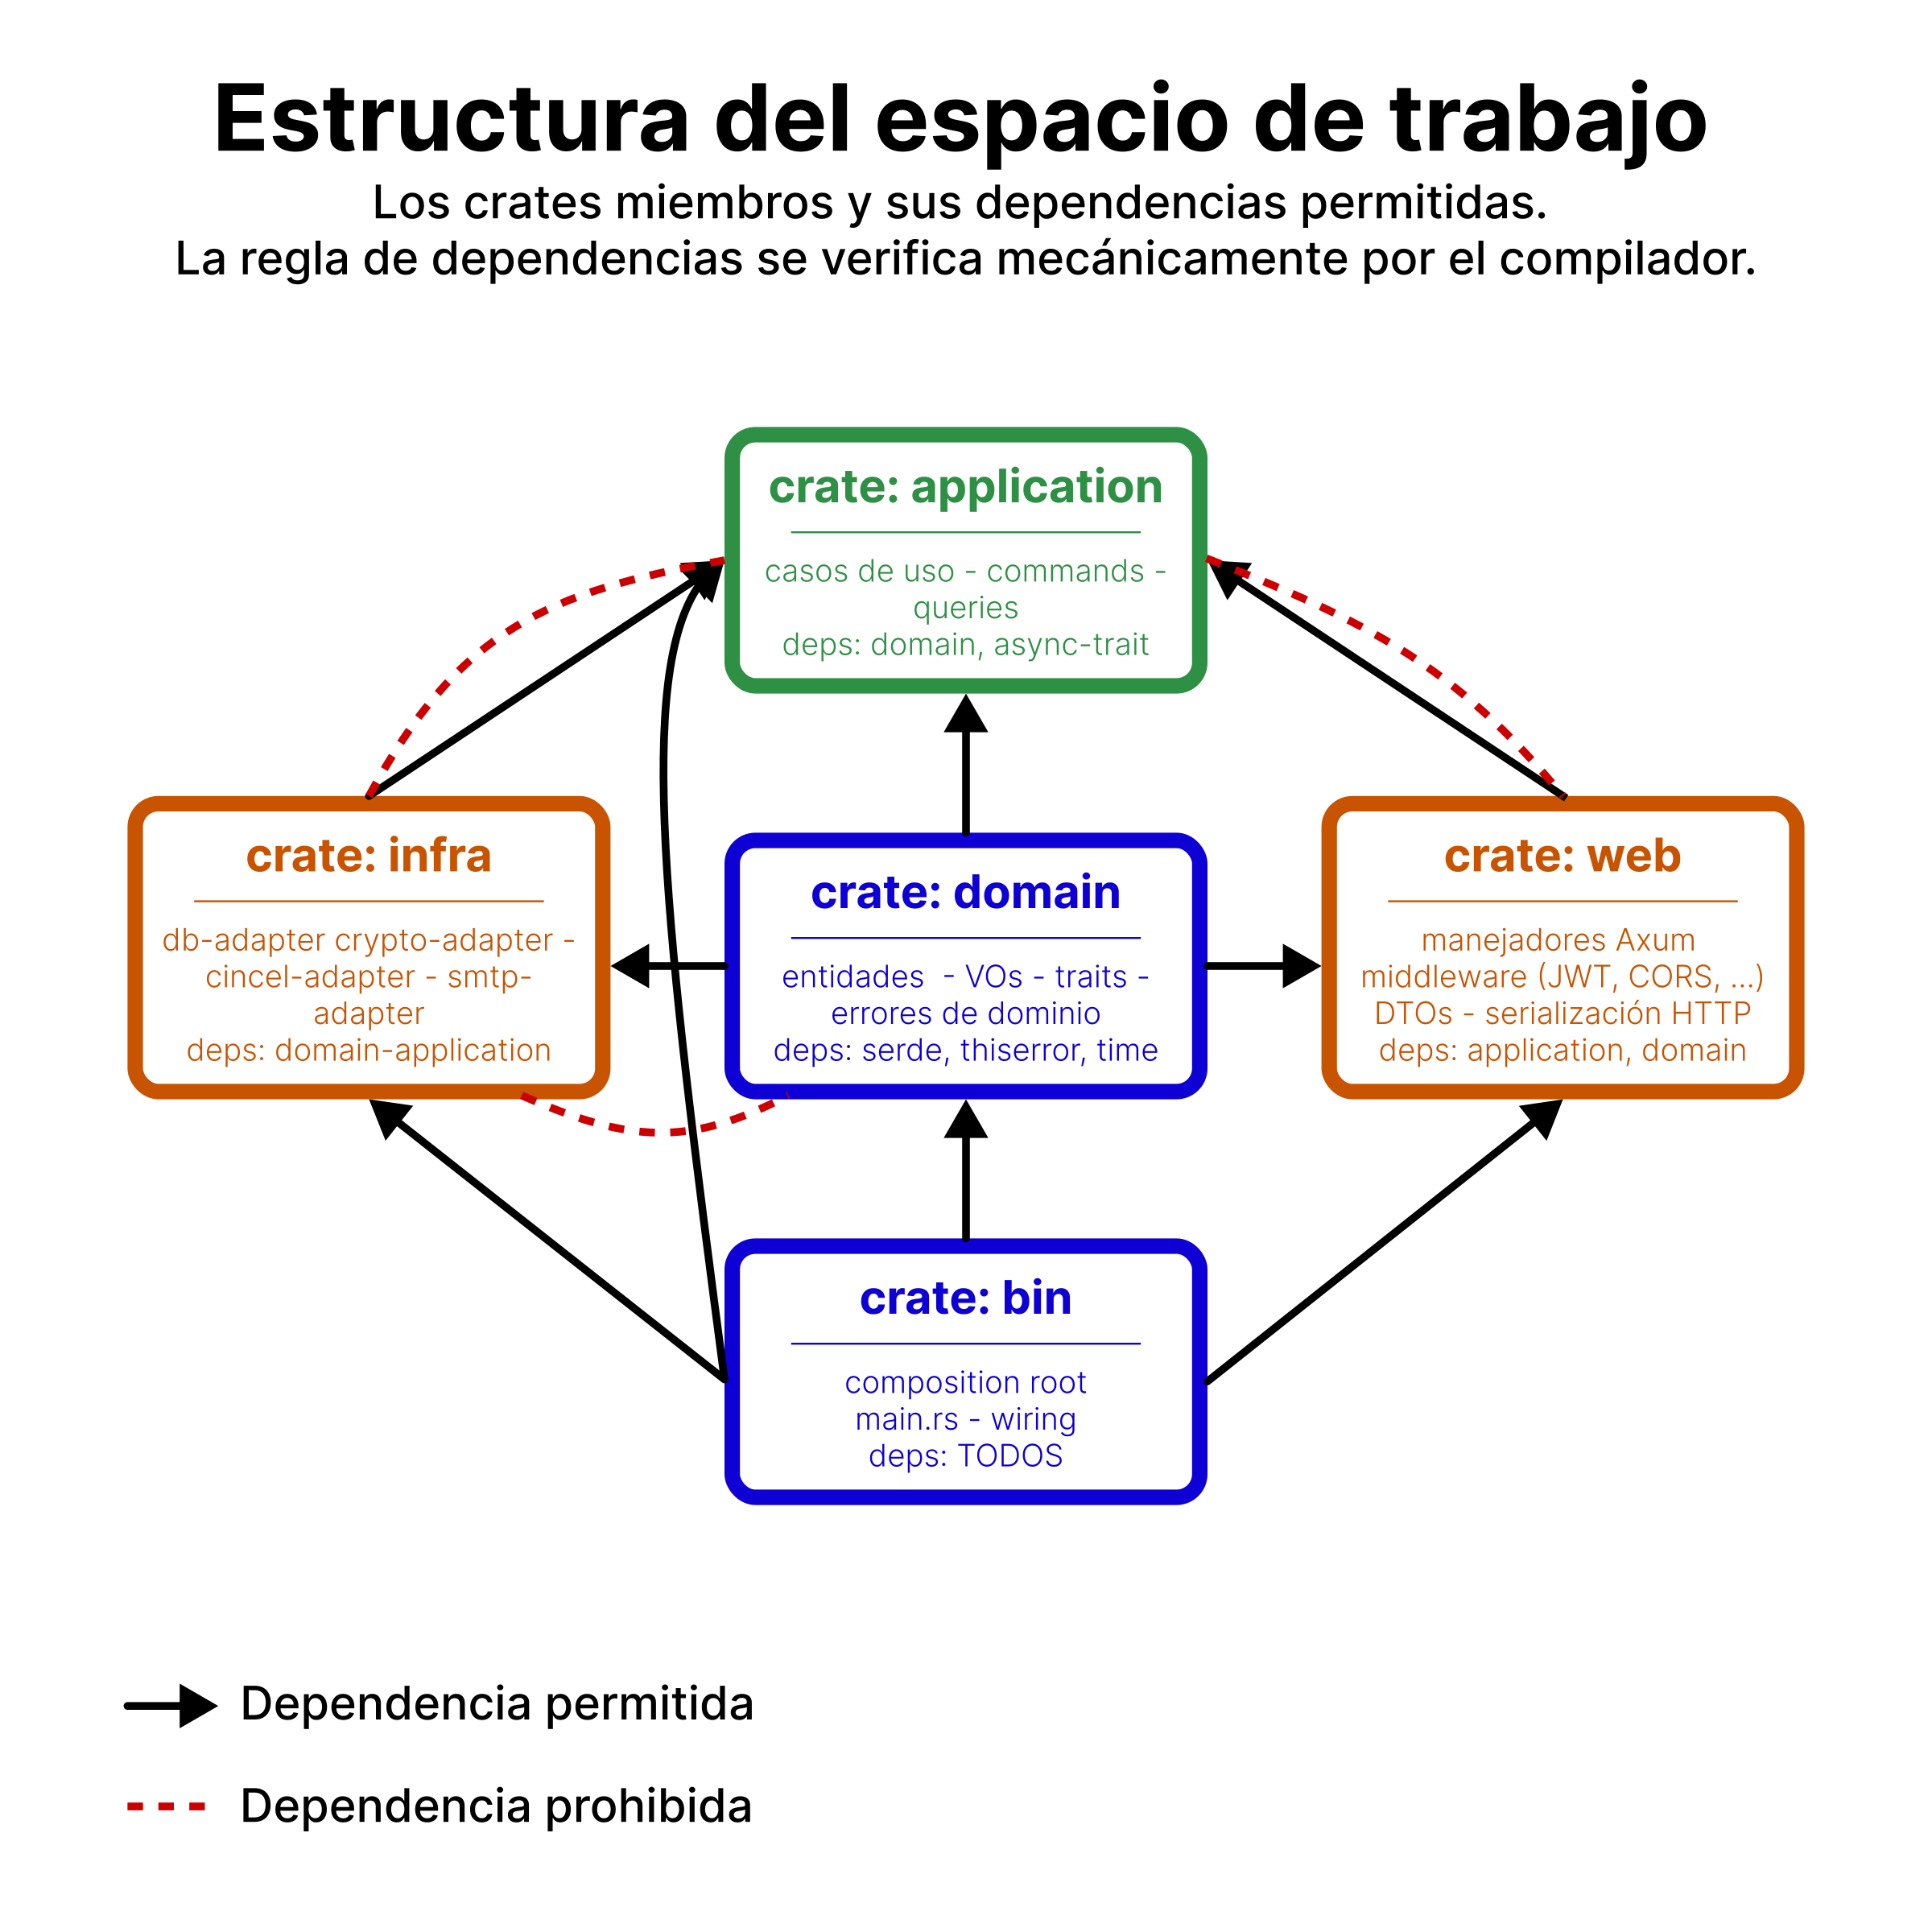
\includegraphics[
        height=0.68\textheight,
        trim=0 500 0 400,
        clip
      ]{workspace.png}
    \end{column}
  \end{columns}
\end{frame}

\begin{frame}{Capacidades criptográficas | primera parte}
  \small
  \begin{tabularx}{\textwidth}{>{\raggedright\arraybackslash\bfseries}p{0.22\textwidth} Y C{0.18\textwidth}}
    \toprule
    Capacidad & Evidencia principal & Estado \\
    \midrule
    Integridad SHA-256 & Hash por bytes y streaming; vectores oficiales y contraste con \texttt{sha256sum}. & \verified \\
    Cifrado autenticado & AES-256-GCM, DEK por documento, KEK envolvente, AAD y rotación. & \verified \\
    PKI interna & CA raíz, certificados RSA-3072, revocación y CRL mediante OpenSSL. & \verified \\
    Firma digital & RSA-3072 con SHA-256 y PKCS\#1 v1.5; interoperabilidad bidireccional. & \verified \\
    Sellado RFC 3161 & TSA local real; adaptador remoto cubierto por stub, sin dependencia de Cincel en la entrega. & \operational \\
    \bottomrule
  \end{tabularx}
\end{frame}

\begin{frame}{Capacidades criptográficas | segunda parte}
  \small
  \begin{tabularx}{\textwidth}{>{\raggedright\arraybackslash\bfseries}p{0.22\textwidth} Y C{0.18\textwidth}}
    \toprule
    Capacidad & Evidencia principal & Estado \\
    \midrule
    Verificación integral & Reporte de integridad, firma, certificado y sello con causas explícitas. & \verified \\
    Credenciales Argon2id & Formato PHC; $m=256$ MiB, $t=4$, $p=1$ y media de 607.8 ms en el host de referencia. & \verified \\
    Segundo factor TOTP & Vectores RFC 6238, ventana de un periodo y códigos de recuperación. & \verified \\
    Auditoría encadenada & Cadena SHA-256 persistida en JSONL y detección del índice alterado. & \verified \\
    Paquete de evidencia & ZIP autocontenido con instrucciones para OpenSSL y \texttt{unzip}. & \verified \\
    \bottomrule
  \end{tabularx}
\end{frame}

\begin{frame}{Estrategia de validación}
  \begin{columns}[T,onlytextwidth]
    \begin{column}{0.23\textwidth}
      \begin{block}{Vectores}
        \small FIPS 180-4, GCM, RFC 6238 y RFC 4226.
      \end{block}
    \end{column}
    \begin{column}{0.23\textwidth}
      \begin{block}{Propiedades}
        \small Entradas generadas, nonces y consistencia de ida y vuelta.
      \end{block}
    \end{column}
    \begin{column}{0.23\textwidth}
      \begin{block}{Mutaciones}
        \small Documento, firma, token, CRL, paquete y bitácora alterados.
      \end{block}
    \end{column}
    \begin{column}{0.23\textwidth}
      \begin{block}{Herramientas}
        \small OpenSSL, \texttt{sha256sum}, \texttt{unzip} y CLI real.
      \end{block}
    \end{column}
  \end{columns}

  \vspace{0.6cm}
  \begin{center}
    \begin{tikzpicture}[node distance=0.25cm]
      \node[draw=linea,fill=white,minimum width=3.0cm,minimum height=0.9cm] (domain) {Dominio};
      \node[draw=linea,fill=white,minimum width=3.0cm,minimum height=0.9cm,right=of domain] (application) {Aplicación};
      \node[draw=linea,fill=white,minimum width=3.0cm,minimum height=0.9cm,right=of application] (infra) {Infraestructura};
      \node[draw=verde,very thick,fill=verde!8,minimum width=3.0cm,minimum height=0.9cm,right=of infra] (e2e) {Extremo a extremo};
      \draw[->,thick,gris] (domain) -- (application);
      \draw[->,thick,gris] (application) -- (infra);
      \draw[->,thick,gris] (infra) -- (e2e);
    \end{tikzpicture}
  \end{center}
  \vspace{0.2cm}
  \centering{\small\color{gris}La prueba observa tanto primitivas aisladas como su composición en un proceso real.}
\end{frame}

\begin{frame}{Resultados de pruebas y cobertura}
  \begin{columns}[T,onlytextwidth]
    \begin{column}{0.63\textwidth}
      \coveragebar{domain}{95.9}{934 / 974 líneas}
      \coveragebar{application}{96.2}{1,137 / 1,182 líneas}
      \coveragebar{infrastructure}{93.5}{1,881 / 2,012 líneas}
      \coveragebar{bin}{88.1}{833 / 946 líneas; valor informativo}
    \end{column}
    \begin{column}{0.33\textwidth}
      \begin{block}{Suite completa}
        \centering
        {\fontsize{28}{30}\selectfont\bfseries 367}\par
        {\small funciones descubiertas}\par
        \vspace{0.3cm}
        {\color{verde}\bfseries 366 aprobadas}\par
        {\color{tinta}0 fallidas}\par
        {\color{advertencia}1 ignorada}
      \end{block}
    \end{column}
  \end{columns}
  \vspace{0.2cm}
  {\scriptsize\color{gris}El umbral del 90\% aplica a los tres crates con lógica criptográfica. La prueba ignorada conserva la sonda del sandbox externo, que no forma parte de la evidencia actual por su inestabilidad y costo no transparente.}
\end{frame}

\begin{frame}[fragile]{Demostración integral reproducida}
  \begin{columns}[T,onlytextwidth]
    \begin{column}{0.52\textwidth}
      \small
      \begin{enumerate}
        \item Crear la CA, el firmante y la TSA local.
        \item Calcular el hash y cifrar con una DEK fresca.
        \item Alterar un byte y comprobar el rechazo autenticado.
        \item Firmar, sellar y verificar los cuatro componentes.
        \item Exportar el ZIP y validarlo con herramientas externas.
        \item Revocar el certificado y ejercitar Argon2id, TOTP y auditoría encadenada.
      \end{enumerate}
    \end{column}
    \begin{column}{0.44\textwidth}
      \begin{lstlisting}[style=terminal]
$ bash scripts/demo.sh

integrity:   passed
signature:   passed
certificate: passed
timestamp:   passed
verdict:     valid

Verified OK
certificado.pem: OK
Verification: OK

All stages finished.
      \end{lstlisting}
    \end{column}
  \end{columns}
\end{frame}

\begin{frame}{Riesgo materializado: dependencia del PSC}
  \begin{columns}[T,onlytextwidth]
    \begin{column}{0.31\textwidth}
      \begin{exampleblock}{Acceso}
        \small El registro en el entorno del proveedor pudo completarse.
      \end{exampleblock}
    \end{column}
    \begin{column}{0.31\textwidth}
      \begin{alertblock}{Operación}
        \small La API no mostró estabilidad suficiente para una campaña repetible.
      \end{alertblock}
    \end{column}
    \begin{column}{0.31\textwidth}
      \begin{alertblock}{Costo}
        \small El sandbox requiere pago y no ofrece precios transparentes para presupuestar una campaña.
      \end{alertblock}
    \end{column}
  \end{columns}

  \vspace{0.3cm}
  \textbf{La materialización no ocurrió en el registro, sino durante el consumo.}
  \begin{itemize}\scriptsize\setlength{\itemsep}{0cm}
    \item Una falla externa puede confundirse con una regresión del adaptador.
    \item La suite y la demostración perderían reproducibilidad.
    \item Los reintentos y la campaña de tokens introducen costo variable.
  \end{itemize}
  \vspace{0.05cm}
  {\scriptsize\color{gris}Estado: TSA local para la evidencia; adaptador remoto opcional y sin contrato externo confirmado.}
\end{frame}

\begin{frame}{Mitigación: TSA interna intercambiable}
  \centering
  \begin{tikzpicture}[
    every node/.style={font=\small,align=center},
    box/.style={draw=linea,fill=white,minimum width=3.1cm,minimum height=0.85cm},
    local/.style={draw=verde,very thick,fill=verde!8,minimum width=3.7cm,minimum height=0.85cm},
    remote/.style={draw=advertencia,very thick,fill=advertencia!8,minimum width=3.7cm,minimum height=0.85cm}
  ]
    \node[box] (usecase) at (0,0) {Caso de uso\\\texttt{TimestampDocument}};
    \node[box] (port) at (4.3,0) {Puerto\\\texttt{TimestampService}};
    \node[local] (local) at (9.2,0.7) {TSA local: OpenSSL + CA interna};
    \node[remote] (remote) at (9.2,-0.7) {PSC externo: Cincel u otro};
    \draw[->,thick,gris] (usecase) -- (port);
    \draw[->,thick,verde] (port) -- (local);
    \draw[->,thick,advertencia] (port) -- (remote);
  \end{tikzpicture}

  \vspace{0.1cm}
  \begin{columns}[T,onlytextwidth]
    \begin{column}{0.55\textwidth}
      \small
      \begin{itemize}
        \item Certificado RSA-3072 exclusivo para \texttt{timeStamping}.
        \item Tokens RFC 3161 reales, no respuestas simuladas.
        \item Verificación independiente con OpenSSL.
      \end{itemize}
    \end{column}
    \begin{column}{0.41\textwidth}
      \begin{alertblock}{Regla operativa}
        \small Sin conmutación silenciosa: el emisor y su ancla de confianza quedan identificados en cada flujo.
      \end{alertblock}
      {\small\color{gris}Pruebas reproducibles sin red ni costo externo.}
    \end{column}
  \end{columns}
\end{frame}

\begin{frame}{Alcance de la mitigación y riesgo residual}
  \begin{columns}[T,onlytextwidth]
    \begin{column}{0.47\textwidth}
      \begin{exampleblock}{La TSA interna sí demuestra}
        \small
        \begin{itemize}
          \item Solicitud y emisión conforme a RFC 3161.
          \item Vinculación del token con el digest.
          \item Firma, cadena y almacenamiento DER.
          \item Interoperabilidad del flujo completo.
        \end{itemize}
      \end{exampleblock}
    \end{column}
    \begin{column}{0.47\textwidth}
      \begin{alertblock}{La TSA interna no sustituye}
        \small
        \begin{itemize}
          \item La independencia de un tercero.
          \item La estabilidad contractual de un PSC.
          \item Una constancia NOM-151 externa.
          \item Una constancia externa que se decida contratar posteriormente.
        \end{itemize}
      \end{alertblock}
    \end{column}
  \end{columns}

  \vspace{0.15cm}
  \centering
  {\small\bfseries\color{tinta}Continuidad técnica demostrada; evidencia externa fuera del alcance actual.}\par
  \vspace{0.08cm}
  {\scriptsize\color{gris}La arquitectura permite sustituir el adaptador sin modificar dominio ni casos de uso.}
\end{frame}


\begin{frame}{Límites abiertos del corte}
  \begin{columns}[T,onlytextwidth]
    \begin{column}{0.31\textwidth}
      \begin{block}{Proveedor de sellado}
        \small La evidencia externa queda fuera del alcance actual. Un PSC futuro requerirá contrato, estabilidad y precios verificables.
      \end{block}
    \end{column}
    \begin{column}{0.31\textwidth}
      \begin{block}{Calibración Argon2id}
        \small $m=256$ MiB, $t=4$, $p=1$: 607.8 ms en el host de referencia, dentro de banda. Repetir si cambia el hardware.
      \end{block}
    \end{column}
    \begin{column}{0.31\textwidth}
      \begin{block}{Web y persistencia}
        \small Implementar API, sesiones, roles, PostgreSQL y Redis sobre los puertos existentes.
      \end{block}
    \end{column}
  \end{columns}

  \vspace{0.3cm}
  \begin{alertblock}{Interpretación}
    \small El núcleo criptográfico está implementado y probado. La TSA local cierra la demostración técnica y Argon2id ya está calibrado en el host de referencia; el frente restante es la integración funcional.
  \end{alertblock}
\end{frame}

\begin{frame}{Resultado del avance}
  \begin{columns}[c,onlytextwidth]
    \begin{column}{0.60\textwidth}
      {\fontsize{19}{23}\selectfont\bfseries\color{tinta}
        El núcleo está listo para integrarse sin trasladar criptografía ni reglas de dominio a la capa web.\par}
      \vspace{0.35cm}
      {\normalsize\color{verde}\bfseries Implementación, evidencia y documentación coinciden en el mismo corte.}
    \end{column}
    \begin{column}{0.36\textwidth}
      \begin{block}{Entregables}
        \small
        \begin{itemize}
          \item Reporte LaTeX actualizado.
          \item Informe de verificación local.
          \item Transcripción de demostración.
          \item PDF de esta presentación.
        \end{itemize}
      \end{block}
    \end{column}
  \end{columns}
  \vspace{0.42cm}
  \centering{\scriptsize\color{gris}\texttt{docs/verification-report.md} \quad | \quad \texttt{scripts/demo.sh}}
\end{frame}

\end{document}
